% Supplementary Information body, shared by main.tex (appendix) and supplement.tex.
\noindent Contents: Supplementary Fig.~\ref{fig:S1} (Fig.~2 supplement: access by format beyond one cell, cross-modal groups, linked contacts), Supplementary Table~\ref{tab:S1} (what each format can represent: definitions, rules and evidence for every cell of Fig.~2b) and Supplementary Table~\ref{tab:S2} (interactive viewers for 3-D genome data compared on ten capabilities).
Methods, datasets and benchmark protocol are described in the main text (Methods).

% ------------------------------------------------------------------ Fig. S1
\begin{figure}[!h]
  \centering
  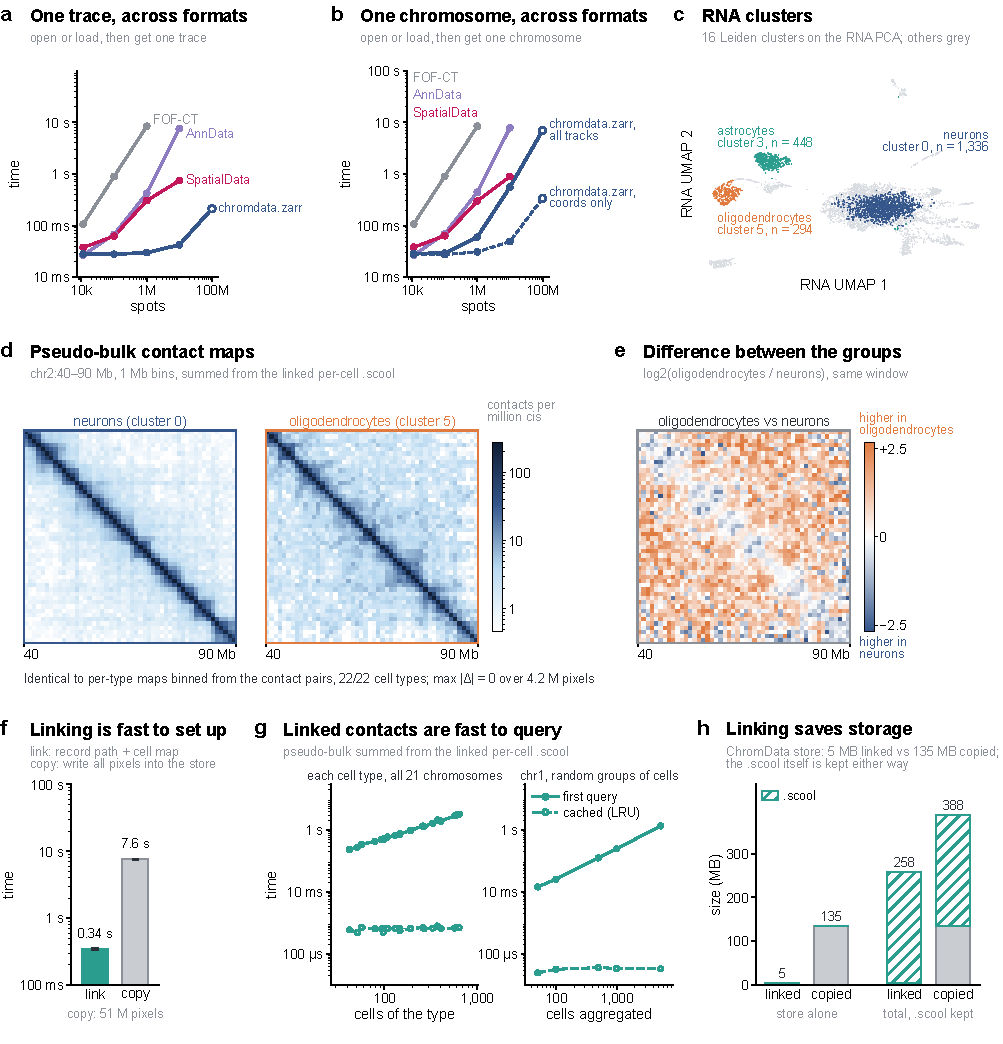
\includegraphics[width=0.84\textwidth]{figS1.pdf}
  \caption[Fig.~2 supplement: access by format, cross-modal groups, linked contacts]{\textbf{Access by format beyond one cell (a, b); groups from one modality, structure from another (c--e); linked contacts: set-up, query speed and storage (f--h).}
\textbf{a,\,b}~Time to open or load the file and get one trace (\textbf{a}) or one chromosome (\textbf{b}), for the data of Fig.~2c~\citep{takei2025}; median of 20 random ids.
At $10^{7}$ spots, one trace: chromdata.zarr 42\,ms, SpatialData 0.74\,s, AnnData 7.6\,s.
One chromosome: chromdata.zarr 0.56\,s with all 62 per-spot tracks (solid) and 49\,ms with coordinates only (dashed), SpatialData 0.89\,s, AnnData 7.8\,s.
FOF-CT stops at $10^{6}$ spots (8.4\,s; memory limit). Open markers, replicated cells (Fig.~2).
\textbf{c--h}~scHiCAR mouse primary motor cortex, 5,313 cells, per-cell 1-Mb contact maps in a linked .scool file~\citep{schicar}.
\textbf{c}~Three of 16 Leiden clusters of the RNA profiles, computed in ChromData (other clusters grey), on the RNA UMAP: oligodendrocytes (cluster~5; \emph{Plp1}, \emph{St18}, \emph{Prr5l}, \emph{Mobp}; $n=294$), astrocytes (cluster~3; \emph{Gpc5}, \emph{Slc1a3}, \emph{Atp1a2}; $n=448$) and neurons (cluster~0; no glial or vascular markers; $n=1{,}336$).
\textbf{d}~Pseudo-bulk contact maps of the neuron and oligodendrocyte clusters, summed from the linked per-cell maps through the shared index (chr2:40--90\,Mb, 1-Mb bins, normalised to cis contacts).
For all 22 published cell types they equal maps binned directly from the contact pairs (4.2\,M pixels, maximum absolute difference 0).
\textbf{e}~$\log_2$(oligodendrocytes\,/\,neurons) of the maps in \textbf{d}.
Away from the diagonal 75\,\% of pixels are higher in oligodendrocytes; the map is noisy at 1\,Mb and illustrates a downstream comparison, not a biological claim.
\textbf{f}~Time to attach the per-cell maps to a store: link (path, bin size, cell map; 0.34\,s) or copy all 51\,M pixels (7.6\,s); whiskers, min--max.
\textbf{g}~Pseudo-bulk query time, first query (filled markers, solid) and the same query again (cached; open markers, dashed).
Left, whole-genome cis maps of each of the 22 cell types against the cells of the type; right, chr1 for random groups of 50 to 5,313 cells.
\textbf{h}~On-disk size. Left, the store alone with the maps linked (5\,MB) or copied (135\,MB). Right, the total footprint, which keeps the community .scool (253\,MB, hatched) either way: 258\,MB linked against 388\,MB copied.
Protocol and machine: Methods.
\unskip}
  \label{fig:S1}
\end{figure}
\clearpage

% ---------------------------------------------------------------- Table S1
\setlength{\LTleft}{0pt}\setlength{\LTright}{0pt plus 1fill}
\footnotesize
\begin{longtable}{@{}l*{12}{c}@{}}
\caption[What each format can represent]{\textbf{What each format can represent (evidence for Fig.~2b).}
Marks as in Fig.~2b: \mNative{}~native, first-class with its own structure; \mLinked{}~linked, kept in an external community-standard file (not copied) and queried through the shared index; \mConv{}~by convention, stored and read back through the library's public API but only in a general-purpose slot (\pkg{uns}, \pkg{obsm}, \pkg{varp}, \pkg{attrs}, metadata attributes, extra or optional columns), so the structure is lost or ad hoc; \mNone{}~not supported, no place for it in the format or its API.
Column definitions, rules and the evidence for every cell follow the matrix.}
\label{tab:S1}\\
\toprule
Container & \rot{spot coordinates (x, y, z)} & \rot{cell › trace › spot hierarchy} & \rot{per-spot signals} & \rot{per-locus (bin) signals} & \rot{cell table} & \rot{cell embeddings} & \rot{cell spatial position} & \rot{contact maps} & \rot{intervals (TADs / loops)} & \rot{non-genomic points (RNA spots)} & \rot{results with provenance} & \rot{partial reads (cell / chrom.)} \\
\midrule
\endfirsthead
\toprule
Container & \multicolumn{12}{c}{(continued)}\\
\midrule
\endhead
\inputrows{supp/tableS1_matrix.tex}
\bottomrule
\end{longtable}

\normalsize
\noindent\textbf{Columns.}
\emph{Spot coordinates (x, y, z)}: the position of every spot (one imaged or reconstructed locus in one trace), with its unit.
\emph{Cell › trace › spot hierarchy}: which trace and which cell each spot belongs to, as nested levels rather than loose labels.
\emph{Per-spot signals}: values measured per spot, such as immunofluorescence intensity or z-scores at that spot.
\emph{Per-locus (bin) signals}: values per genomic bin shared by all cells, such as bulk ATAC / ChIP tracks or GC content.
\emph{Cell table}: scalar properties per cell, such as cell type, volume or RNA counts.
\emph{Cell embeddings}: a multi-dimensional vector per cell, such as a PCA, UMAP or learned embedding.
\emph{Cell spatial position}: where each cell is in the tissue or field of view (centroid and / or outline), with unit and coordinate frame.
\emph{Contact maps}: locus~$\times$~locus contact counts (Hi-C-type maps), in bulk or per cell.
\emph{Intervals}: genomic intervals and interval pairs called on the data, such as TADs and loops.
\emph{Non-genomic points}: 3-D points that are not genomic loci, such as RNA spots or protein puncta.
\emph{Results with provenance}: analysis results stored as data together with the function, parameters and version that produced them.
\emph{Partial reads}: reading one cell's or one chromosome's rows from disk without reading the rest of the data.

\medskip\noindent\textbf{Rules.}
(1)~The evidence decides; only where it is genuinely ambiguous does the other tool get the better mark, and the note starts with \emph{Judgement call}.
(2)~AnnData and MuData are rated in their most favourable orientation (spots, cells or loci as observations), and these orientations exclude each other in one object (one AnnData, one MuData modality; a MuData can hold one modality per orientation, linked only by \pkg{obs} columns). The hierarchy column is where that shows; the same holds for a SpatialData table, which is an AnnData.
(3)~A test that needed a general-purpose slot can back at most \emph{by convention}, one that needed an external file \emph{linked}; the audit fails on any mismatch between a mark and its test.
(4)~A data table serialised to JSON text inside a descriptive metadata attribute (cooler's \pkg{metadata}) does not count; such tests are still run and reported as \emph{not counted}. Parameter and software records (provenance) there do count, and so do scalar key--values that describe the object carrying the attribute (each cell's own cooler in a .scool), as a general-purpose slot; the result itself must be stored as data.
(5)~\emph{Partial reads}: native when one cell's or one chromosome's rows are read from disk without reading the other rows (beyond the selection key column); by convention when that is only possible by scanning every row (streamed, memory bounded) or with part of the data (e.g.\ \pkg{obs} / \pkg{obsm}) loaded whole.
(6)~\emph{By convention} needs a normal use of the format that only lacks the dedicated structure; an encoding that merely writes (tracing traces as per-trace column sets of cooler bins tables, an embedding split into one metadata key per dimension) is rated \emph{not supported}, and its test is still reported.

\medskip\noindent\textbf{Tests.}
Every library cell was verified by a store-and-read-back test: a tiny object stored the element with that library's own API, was written to disk, read back and compared; the slot it used (dedicated, general-purpose or external) is given in the last column below.
FOF-CT is a CSV specification, not a library, so its row rests on the specification pages alone (core, trace, cell, mapping, bio, quality, rna, subcell and the format overview)~\citep{fofct}.
The test code is available in the code repository (Methods, Code availability).

\medskip\noindent\textbf{Versions checked.}
AnnData 0.12.11~\citep{anndata}; SpatialData 0.7.2~\citep{spatialdata}; MuData 0.3.4~\citep{mudata}; cooler 0.10.4~\citep{cooler}; zarr 3.1.6~\citep{zarr}; h5py 3.16.0; FOF-CT v1.0 (specification pages checked 2026-09-27).

\medskip\noindent\textbf{Judgement calls:} AnnData, partial reads; SpatialData, per-locus signals (see the evidence below).

\bigskip\noindent\textbf{Changes after the audits.}
\begingroup\footnotesize
\begin{longtable}{@{}>{\raggedright\arraybackslash}p{0.13\textwidth}>{\raggedright\arraybackslash}p{0.17\textwidth}>{\raggedright\arraybackslash}p{0.10\textwidth}>{\raggedright\arraybackslash}p{0.10\textwidth}>{\raggedright\arraybackslash}p{0.34\textwidth}@{}}
\toprule
Container & Element & Before & After & Reason \\
\midrule
\endhead
\inputrows{supp/tableS1_changes.tex}
\bottomrule
\end{longtable}
\addtocounter{table}{-1}  % longtable steps the table counter even without a caption: this one is part of Table S1
\endgroup

\begingroup\footnotesize
\noindent\textbf{Evidence per cell.} Documentation links are given as URLs; ``dedicated'', ``general-purpose'' and ``external'' name the slot the store-and-read-back test used.
\begin{longtable}{@{}>{\raggedright\arraybackslash}p{0.17\textwidth}>{\raggedright\arraybackslash}p{0.12\textwidth}>{\raggedright\arraybackslash}p{0.38\textwidth}>{\raggedright\arraybackslash}p{0.23\textwidth}@{}}
\toprule
Element & Mark & Evidence & Store-and-read-back test \\
\midrule
\endfirsthead
\toprule
Element & Mark & Evidence & Store-and-read-back test \\
\midrule
\endhead
\bottomrule
\endfoot
\inputrows{supp/tableS1_evidence.tex}
\end{longtable}
\addtocounter{table}{-1}  % longtable steps the table counter even without a caption: this one is part of Table S1
\endgroup

% ---------------------------------------------------------------- Table S2
% Viewers compared on ten capabilities.  Every mark comes from the tool's papers, documentation or code
% (checked 2026-10-05); the notes give the reason for every partial mark and for the less obvious others.
\clearpage
\setlength{\LTleft}{0pt}\setlength{\LTright}{0pt plus 1fill}
\footnotesize
\newcommand{\N}{\mNative{}}\newcommand{\Pt}{\mPartial{}}\newcommand{\X}{\mNone{}}
\begin{longtable}{@{}l*{10}{c}@{}}
\caption[Interactive viewers for 3-D genome data]{\textbf{Interactive viewers for 3-D genome data.}
Fourteen published viewers and U-Chrom rated on ten capabilities, from each tool's papers, documentation and code (checked 2026-10-05).
\mNative{}~native: built in and documented; \mPartial{}~partial: limited as stated in the notes below the table; \mNone{}~not found in the papers, documentation or code.
Columns and rules follow the table.}
\label{tab:S2}\\
\toprule
Viewer & \rot{bulk contact maps} & \rot{per-cell contact maps (scHi-C)} & \rot{per-spot maps (spatial Hi-C)} & \rot{chromatin tracing (many traces)} & \rot{3-D structures} & \rot{genomic tracks} & \rot{cell embedding or table} & \rot{cell or spot positions} & \rot{views linked by locus} & \rot{views linked by cell selection} \\
\midrule
\endfirsthead
\toprule
Viewer & \multicolumn{10}{c}{(continued)}\\
\midrule
\endhead
\multicolumn{11}{@{}l}{\emph{Contact-map browsers}}\\
HiGlass~\citep{higlass} & \N & \X & \X & \X & \X & \N & \X & \X & \N & \X \\
Juicebox.js~\citep{juiceboxjs} & \N & \X & \X & \X & \X & \N & \X & \X & \N & \X \\
3D Genome Browser 2.0~\citep{threedgb2} & \N & \Pt & \X & \X & \X & \N & \X & \X & \N & \X \\
WashU Epigenome Browser~\citep{washu2022,washu3d,washu2025} & \N & \Pt & \X & \X & \N & \N & \X & \X & \N & \X \\[2pt]
\multicolumn{11}{@{}l}{\emph{3-D structure viewers}}\\
HiCube~\citep{hicube} & \N & \X & \X & \X & \N & \N & \X & \X & \N & \X \\
4D Genome Browser~\citep{fourdgb} & \N & \X & \X & \X & \N & \Pt & \X & \X & \N & \X \\
ChromPolymerDB~\citep{chrompolymerdb} & \N & \X & \X & \X & \N & \N & \X & \X & \Pt & \X \\
ChromoSkein (preprint)~\citep{chromoskein} & \X & \X & \X & \X & \N & \N & \X & \X & \N & \X \\[2pt]
\multicolumn{11}{@{}l}{\emph{Chromatin-tracing viewers}}\\
Spacewalk~\citep{spacewalk} & \N & \X & \X & \N & \N & \N & \X & \X & \Pt & \X \\
OLIVE~\citep{olive} & \X & \X & \X & \N & \N & \X & \X & \X & \Pt & \X \\[2pt]
\multicolumn{11}{@{}l}{\emph{Multimodal and single-cell viewers}}\\
Nucleome Browser~\citep{nucleomebrowser} & \N & \Pt & \X & \Pt & \N & \N & \X & \Pt & \N & \X \\
Vitessce~\citep{vitessce} & \Pt & \X & \X & \X & \X & \N & \N & \N & \Pt & \Pt \\
SGS genome browser~\citep{sgs} & \N & \Pt & \X & \X & \X & \N & \N & \N & \N & \Pt \\
Higashi visualization~\citep{higashi} & \Pt & \N & \X & \X & \X & \X & \N & \X & \Pt & \N \\[2pt]
\midrule
U-Chrom (this work) & \N & \N & \N & \N & \N & \N & \N & \N & \Pt & \N \\
\bottomrule
\end{longtable}

\normalsize
\noindent\textbf{Columns.}
\emph{Bulk contact maps}: Hi-C-type contact matrices from files such as .hic, .cool or .mcool.
\emph{Per-cell contact maps}: the maps of many single cells held together, with a cell or a group of cells chosen to show its map or the sum of the group's maps.
\emph{Per-spot maps}: the contact maps of the spots of a tissue section, tied to the spots' positions.
\emph{Chromatin tracing}: imaged 3-D traces of many cells loaded as data.
\emph{3-D structures}: chromatin structures or traces drawn in 3-D.
\emph{Genomic tracks}: 1-D signals along the genome.
\emph{Cell embedding or table}: a cell embedding (such as a UMAP) or a cell table in which cells can be selected.
\emph{Cell or spot positions}: cells or spots drawn at their positions in a tissue section, field of view or image.
\emph{Views linked by locus}: navigating the genome in one view moves the other views (maps, tracks and 3-D).
\emph{Views linked by cell selection}: selecting cells in an embedding or in space re-scopes the contact maps, tracks or 3-D views to those cells.

\medskip\noindent\textbf{Rules.}
(1)~Each tool is rated on its own; a feature of a separate application built around it counts for that application (Vitessce embeds HiGlass, Spacewalk embeds juicebox.js and igv.js), and a viewer built only for one figure of a paper counts as partial.
(2)~Per-cell contact maps count only when a paper or the documentation shows per-cell or per-group maps of a single-cell data set; a statement that a file format could hold them does not.
(3)~A map computed by the viewer from 3-D coordinates is a distance or contact map of those coordinates, not a contact map in the first column.
(4)~Linking by cell selection needs a cell embedding, cell table or spatial view to select in; stepping through traces, alleles or models by number is noted but not counted.
(5)~Where two readings were possible, the stricter mark was given and the note says so.

\medskip\noindent\textbf{Notes.}
\emph{HiGlass}: higlass.js 2.3.5; no cell, trace or 3-D data type in the core or the official plugins.
\emph{Juicebox.js}: v4.9.0; its paper notes that a .hic file can hold a single cell's map, but the viewer has no cell collection or cell selection (rule~2).
\emph{3D Genome Browser 2.0}: the single-cell data are cell-type pseudo-bulk maps computed in advance and loaded as ordinary .mcool data sets; per-cell maps are named as future work; no 3-D rendering despite the name.
\emph{WashU Epigenome Browser}: a dynamic Hi-C track steps through a fixed set of maps, also of single cells, without selecting or summing cells (partial); 3-D models (g3d, also of several cells) are drawn with 3Dmol.js and stay in step with the browser region; the image track shows microscopy images by genomic locus, not cell positions.
\emph{HiCube}: two cases side by side; the 3-D view shows one cell's model of a g3d file.
\emph{4D Genome Browser}: two structures from polymer simulation of bulk Hi-C; tracks are per-bead values painted on the structure and plotted for a selection only (partial).
\emph{ChromPolymerDB}: its single-cell structures are inferred from bulk Hi-C, not measured; one locus query sets all views (partial).
\emph{ChromoSkein}: arXiv preprint only; its 2-D map is a distance map of the 3-D model (rule~3); tracks from BED files.
\emph{Spacewalk}: release r15.33, no paper; contact and distance maps of the loaded traces are computed live; one trace is drawn at a time and picked by number (rule~4); hovering a track or the map highlights the region in 3-D, but all panels stay on the locus of the loaded traces (partial).
\emph{OLIVE}: one allele at a time, chosen from lists by field of view and allele; clicking the distance map highlights a readout pair in 3-D (partial).
\emph{Nucleome Browser}: eight single-cell Hi-C maps were shown as separate tracks (partial); chromatin traces and microscopy images of a chosen cell were shown in viewers built for the paper (partial); views share the viewed and highlighted genomic regions; the core platform passes no cell selection between views.
\emph{Vitessce}: v4.0.10; contact maps only through an undocumented generic HiGlass view (partial); genomic profiles are computed in advance per cell set, and a selection colours them without re-computing them (partial); only the HiGlass-based views follow the genomic position (partial); 3-D views are for image volumes and segmentations.
\emph{SGS genome browser}: Hi-C as .hic tracks computed per cell type (partial); a cell selection re-scopes the single-cell ATAC tracks but not the contact maps (partial).
\emph{Higashi visualization}: reads Higashi's own output only; all cells give a pseudo-bulk but no bulk file can be loaded (partial); a selection in the embedding shows the summed maps of the selected cells; map panels share their ranges, set by bin sliders (partial).
\emph{U-Chrom}: tracks are the signals of the store (per spot, per locus, cell~$\times$~bin matrices), not bigWig files; the Genome, Matrix and Stats views share the locus, but the 3-D view does not follow it (a region is highlighted there separately), hence partial.

\medskip\noindent\textbf{Checked and not listed.}
Tools with no interactive view (Fast-Higashi, scHiCTools, pyHiM), libraries and grammars without an application (Uchimata, the Gosling 3-D grammar), tools without cell-level data that duplicate rows above (4DN Data Portal, which uses HiGlass; CSynth, GenomeFlow, Delta, HiBrowser), and unpublished code (napari-nucleome).
The spatial Hi-C studies whose data are in the atlas (Chen et al.\ 2026, Wang et al.\ 2026, Guo et al.\ 2026) do not provide an interactive viewer.

